\documentclass[color=usenames,dvipsnames]{beamer}\usepackage[]{graphicx}\usepackage[]{color}
% maxwidth is the original width if it is less than linewidth
% otherwise use linewidth (to make sure the graphics do not exceed the margin)
\makeatletter
\def\maxwidth{ %
  \ifdim\Gin@nat@width>\linewidth
    \linewidth
  \else
    \Gin@nat@width
  \fi
}
\makeatother

\definecolor{fgcolor}{rgb}{0.345, 0.345, 0.345}
\newcommand{\hlnum}[1]{\textcolor[rgb]{0.686,0.059,0.569}{#1}}%
\newcommand{\hlstr}[1]{\textcolor[rgb]{0.192,0.494,0.8}{#1}}%
\newcommand{\hlcom}[1]{\textcolor[rgb]{0.678,0.584,0.686}{\textit{#1}}}%
\newcommand{\hlopt}[1]{\textcolor[rgb]{0,0,0}{#1}}%
\newcommand{\hlstd}[1]{\textcolor[rgb]{0.345,0.345,0.345}{#1}}%
\newcommand{\hlkwa}[1]{\textcolor[rgb]{0.161,0.373,0.58}{\textbf{#1}}}%
\newcommand{\hlkwb}[1]{\textcolor[rgb]{0.69,0.353,0.396}{#1}}%
\newcommand{\hlkwc}[1]{\textcolor[rgb]{0.333,0.667,0.333}{#1}}%
\newcommand{\hlkwd}[1]{\textcolor[rgb]{0.737,0.353,0.396}{\textbf{#1}}}%
\let\hlipl\hlkwb

\usepackage{framed}
\makeatletter
\newenvironment{kframe}{%
 \def\at@end@of@kframe{}%
 \ifinner\ifhmode%
  \def\at@end@of@kframe{\end{minipage}}%
  \begin{minipage}{\columnwidth}%
 \fi\fi%
 \def\FrameCommand##1{\hskip\@totalleftmargin \hskip-\fboxsep
 \colorbox{shadecolor}{##1}\hskip-\fboxsep
     % There is no \\@totalrightmargin, so:
     \hskip-\linewidth \hskip-\@totalleftmargin \hskip\columnwidth}%
 \MakeFramed {\advance\hsize-\width
   \@totalleftmargin\z@ \linewidth\hsize
   \@setminipage}}%
 {\par\unskip\endMakeFramed%
 \at@end@of@kframe}
\makeatother

\definecolor{shadecolor}{rgb}{.97, .97, .97}
\definecolor{messagecolor}{rgb}{0, 0, 0}
\definecolor{warningcolor}{rgb}{1, 0, 1}
\definecolor{errorcolor}{rgb}{1, 0, 0}
\newenvironment{knitrout}{}{} % an empty environment to be redefined in TeX

\usepackage{alltt}
%\documentclass[color=usenames,dvipsnames,handout]{beamer}

%\usepackage[roman]{../pres1}
\usepackage[sans]{../pres1}
\usepackage{graphicx}
\usepackage{bm}
\usepackage{changepage}
\usepackage{tikz}
\usetikzlibrary{shapes,arrows,decorations,backgrounds}
%\usepackage[usenames,dvipsnames]{color}
\usepackage{animate}





\IfFileExists{upquote.sty}{\usepackage{upquote}}{}
\begin{document}

\begin{frame}[plain]
  \begin{center}
    {\huge Metapopulation models \\}
%    \vspace{0.5cm}
%    { \Large Feb 27 \& March 4, 2019} \\
    \vfill
%    \fbox{
      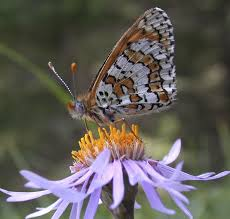
\includegraphics[height=4.2cm,keepaspectratio]{figs/frit} \hspace{0.5cm}
      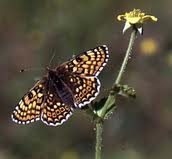
\includegraphics[height=4.2cm,keepaspectratio]{figs/frit2}
%      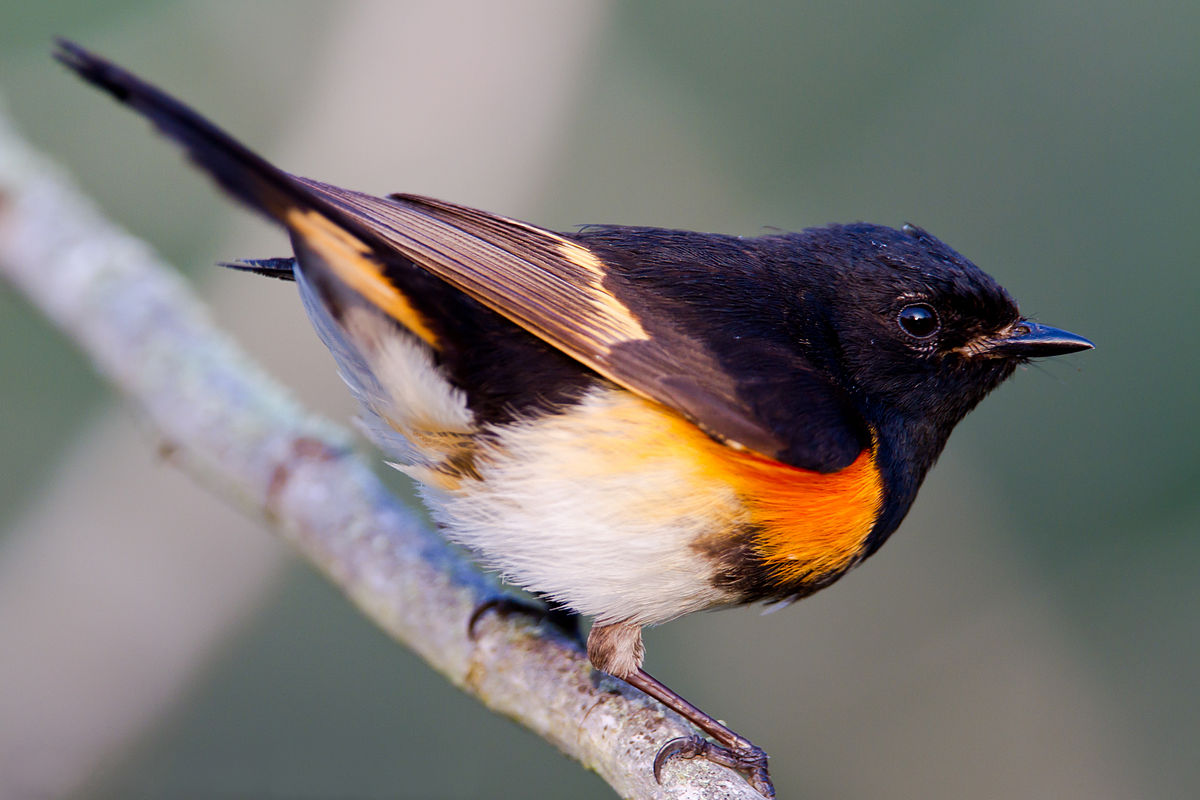
\includegraphics[height=2.8cm,keepaspectratio]{figs/AMRE-ASY-M}
%    }
  \end{center}
\end{frame}



\section{Introduction}


\begin{frame}
  \frametitle{Metapopulations}
  \large
  \begin{center} \Large
    A {\color{TealBlue}
      \bf metapopulation} is a population of
    subpopulations linked by dispersal
  \end{center}
  \pause
  {\bf Properties}
  \begin{itemize}
    \item Subpopulations occur in discrete habitat patches
    \item The landscape ``matrix'' is not suitable for reproduction
  \end{itemize}
\end{frame}


\begin{frame}
  \frametitle{Motivation}
  \large
  \begin{columns}
    \begin{column}{0.6\textwidth}
      \begin{itemize}[<+->]
        \item Many populations are fragmented
        \item Metapopulation models can be used to forecast dynamics of
          fragmented populations
        \item Models can be used to identify critical habitat patches or
          locations for establishing new subpopulations
      \end{itemize}
    \end{column}
    \begin{column}{0.4\textwidth}
      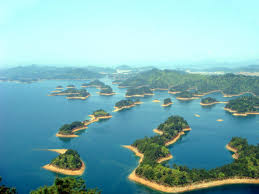
\includegraphics[width=\textwidth]{figs/ping-ding} \\
      \vspace{1cm}
      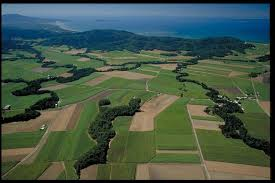
\includegraphics[width=\textwidth]{figs/fragmentation} \par
    \end{column}
  \end{columns}
\end{frame}





\section{Abundance models}



\begin{frame}
  \frametitle{Origins}
  \begin{columns}
    \begin{column}{0.3\textwidth}
      Richard Levins \\
      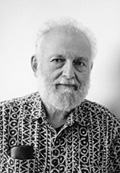
\includegraphics[width=\textwidth]{figs/levins}
    \end{column}
    \begin{column}{0.7\textwidth}
      {\bf First metapopulation models were parameterized in terms of the
        \alert{proportion of patches occupied} \par}
%      \begin{itemize}
%        \item The \alert{state variable} is the proportion of patches occupied
%      \end{itemize}
      \pause
      \vspace{1cm}
      {\bf Modern models are formulated in terms of patch-specific
        \alert{occupancy} or \alert{abundance} \par}
%      {\bf Limitations}
%      \begin{itemize}
%        \item Non-spatial (or spatially implicit)
%        \item Deterministic
%        \item All patches are the same
%      \end{itemize}
    \end{column}
  \end{columns}
\end{frame}







\begin{frame}
  \frametitle{Abundance formulation}
  \Large
  {\centering \bf A simple case with only three subpopulations \par}
  \[
    N_t = n_{1,t} + n_{2,t} + n_{3,t}
  \]
\end{frame}





\begin{frame}
  \frametitle{Abundance and movement}
  \tikzstyle{level 1} = [circle, draw, text width=1cm, minimum size=2cm,
    node distance=4cm, text centered, fill=blue!10]
    \begin{center}
      \begin{tikzpicture}
        \node [level 1] (n1) [xshift=-20mm] {$n_{1,t}$};
        \node [level 1, below of=n1] (n2) [xshift=30mm] {$n_{2,t}$};
        \node [level 1, right of=n1] (n3) [xshift=20mm] [xshift=0mm] {$n_{3,t}$};
        \draw[->,thick] (n1) to [bend right=15] node[left] {$\pi_{1,2}$} (n2);
        \draw[->,thick] (n2) to [bend right=15] node[right] {$\pi_{2,1}$} (n1);
        \draw[->,thick] (n1) to [bend right=15] node[above] {$\pi_{1,3}$} (n3);
        \draw[->,thick] (n3) to [bend right=15] node[above] {$\pi_{3,1}$} (n1);
        \draw[->,thick] (n2) to [bend right=15] node[right] {$\pi_{2,3}$} (n3);
        \draw[->,thick] (n3) to [bend right=15] node[left] {$\pi_{3,2}$} (n2);
        % \draw[->,thick] (n2) to node[above] {$s_2$} (n3);
        % \draw[->,thick] (n2) to [bend right=40] node[above] {$s_2
        % \times b_2$} (n1); \draw[->,thick] (n3) to [bend right=60]
        % node[above] {$s_3 \times b_3$} (n1);
      \end{tikzpicture}
    \end{center}
    The movement probabilities ($\pi_{i,j}$) indicate the proportion of
    individuals moving from patch $i$ to patch $j$
\end{frame}




\begin{frame}
  \frametitle{Abundance models}
  {\centering \bf \large Building the metapopulation model for the first
    subpopulation \par}
  \large
  \[
    n_{1,t+1} = n_{1,t}\lambda_1 \uncover<2->{\color{Blue}{(1 - \pi_{1,2} - \pi_{1,3})} +}
    \uncover<3->{\color{Red}{n_{2,t}\lambda_2 (\pi_{2,1}) + n_{3,t}\lambda_3 (\pi_{3,1})}}
  \]
  \large
  {\bf Three components}
  \begin{enumerate}[\bf (1)]
    \item<1-> Geometric growth
    \item<2-> \color{Blue}{1 minus emigration rates}
    \item<3-> \color{Red}{Immigration from subpopulations 2 and 3}
  \end{enumerate}
\end{frame}



\begin{frame}
  \frametitle{What influences movement?}
  The movement probabilities ($\pi_{i,j}$) represent the outcomes of
  both immigration and emigration.
  \vfill
  What influences these probabilities?
  \pause
  \vfill
  Examples
  \begin{itemize}
    \item Habitat quality in the patch of origin
    \item Habitat quality in the landscape between origin and
      destination patches
    \item Habitat quality in the destination patch
    \item Distance between patches
  \end{itemize}
\end{frame}



\begin{frame}
  \frametitle{Sources, sinks, and traps}
  {\bf Source \\}
  A patch with $\lambda>1$. Sources tend to be net exporters of individuals.  
  \pause
  \vfill
  {\bf Sink \\}
  A patch with $\lambda<1$. Sinks would go extinct in the absence of immigration.
  \pause
  \vfill
  {\bf Ecological trap \\}
  A sink that animals incorrectly perceive as a high quality source.
\end{frame}



\begin{frame}
  \frametitle{Density and habitat quality}
  Can we identify sources, sinks, and traps by estimating
  patch-specific density (at one point in time)? \\
  \pause
  \vfill
  \begin{columns}
    \wide
    \centering
    \fbox{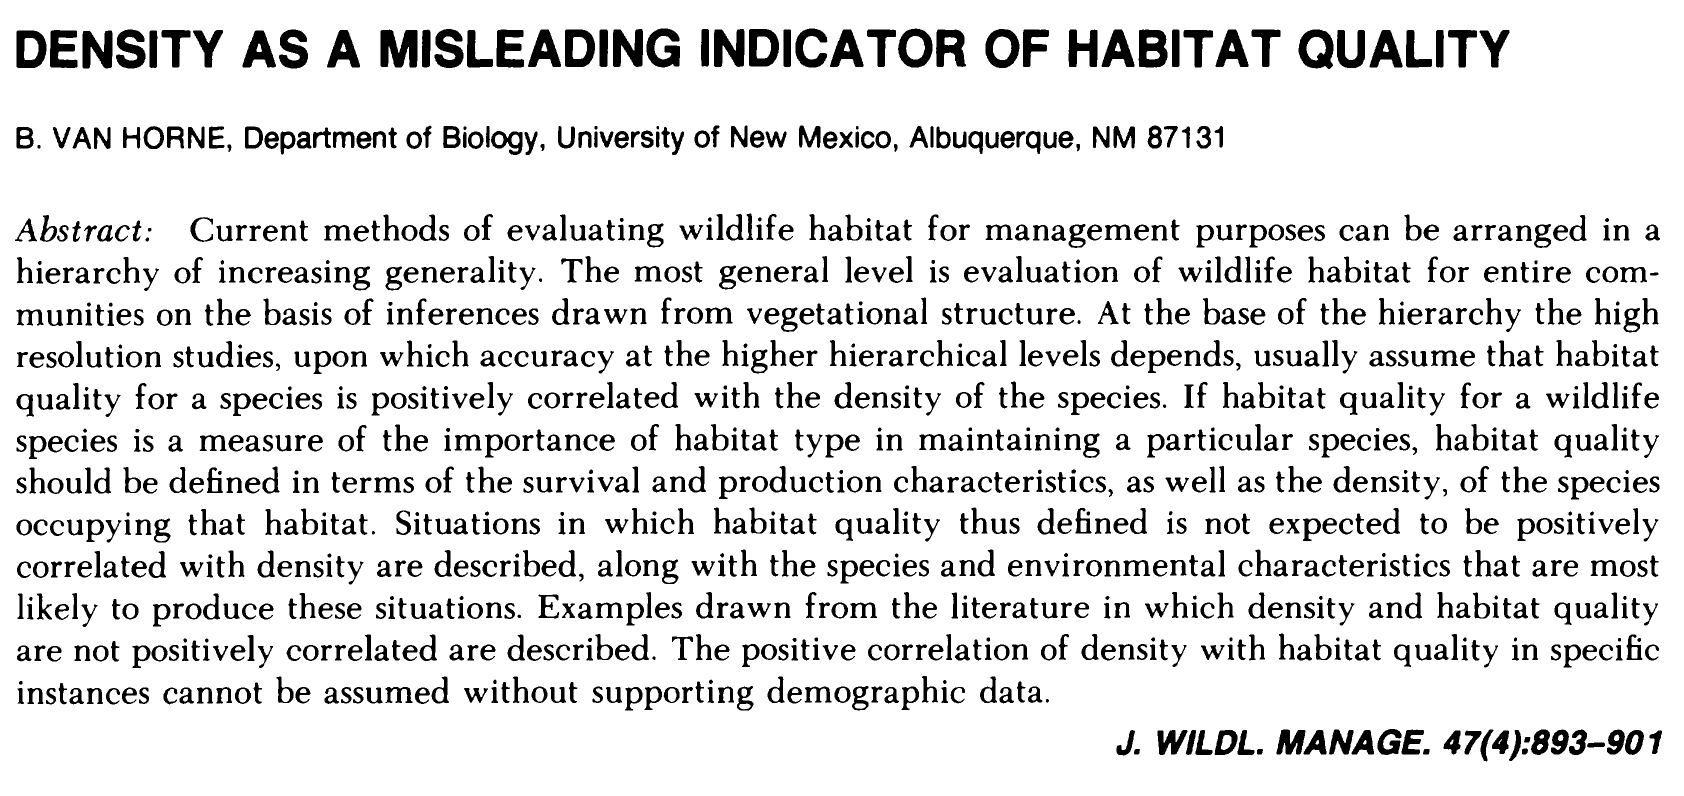
\includegraphics[width=0.95\textwidth]{figs/vanhorne_1983}} \\
  \end{columns}
  \pause
  \vfill
  \centering
  \large
  \alert{\bf Assignment}: Read this paper and be prepared to discuss it \\
\end{frame}




%\section{Non-spatial model}
%\section{Deterministic}
\section{Occupancy models}


\begin{frame}[plain]
  \Huge
  \centering
  \vfill
  \bf 
  \color{MidnightBlue}
  Occupancy models \\
  \vfill
\end{frame}


\begin{frame}[fragile]
  \frametitle{Occupancy models}
  \large
  {\bf Emphasis on stochastic patch-level dynamics}
  \begin{itemize}[<+->]
    \item What is the probability that a patch will be occupied?
    \item What is the probability that an empty patch will be colonized?
    \item What is the probability that a subpopulation will go locally extinct?
    \item What is the probability that the entire metapopulation will
      go extinct?
  \end{itemize}
\end{frame}



\begin{frame}
  \frametitle{Definitions}
  {\bf Occurrence} ($O_{i,t}$) \\
  Indicates if patch $i$ occupied at time $t$  \\
  \pause
  \vfill
  {\bf Occurrence probability} (psi=$\psi_{i,t}$) \\
  Probability that site $i$ is occupied at time $t$
  \pause
  \vfill
  {\bf Colonization probability} (gamma=$\gamma$) \\
  The probability that an unoccupied patch at time $t$ becomes occupied
  at time $t+1$ \par
  \pause
  \vfill
  {\bf Local extinction probability} (epsilon=$\varepsilon$) \\
  The probability that an occupied patch at time $t$ becomes
  unoccupied at time $t+1$ \par
  \pause
  \vfill
  {\bf Metapopulation extinction risk} \\
  The probability that all subpopulation will go extinct
\end{frame}




\begin{frame}[fragile]
  \frametitle{Example}
  \vspace{-1cm}

\includegraphics[width=0.99\textwidth]{figs/ex1/ex1-1}
\end{frame}



\begin{frame}[fragile]
  \frametitle{Example}
\begin{knitrout}
\definecolor{shadecolor}{rgb}{0.969, 0.969, 0.969}\color{fgcolor}

\includegraphics[width=\maxwidth]{figure/ex2-1} \hfill{}



\end{knitrout}
\end{frame}







\begin{frame}
  \frametitle{The model}
  \[
    \psi_{i,t+1} = O_{i,t}(1-\varepsilon) + (1-O_{i,t})\gamma
  \]
  \uncover<2>{
  \[
    O_{i,t+1} \sim \mbox{Bernoulli}(\psi_{i,t+1})
  \]
  } \\
%  where \\
  \vspace{0.5cm}
  \rule{0.5\textwidth}{1pt} \\
  $O_{i,t}$=1 if patch $i$ is occupied at time $t$ \\
  $O_{i,t}$=0 if patch $i$ is unoccupied at time $t$ \\
  $\psi_{i,t}$ is probability that patch $i$ will be occupied at time
  $t$ \\
  $\varepsilon$ is local extinction probability \\
  $\gamma$ is colonization probability
\end{frame}



\begin{frame}
  \frametitle{Assumptions of basic non-spatial model}
  \Large
  \begin{itemize}
    \item Abundance doesn't matter
    \item Patch quality is constant
    \item Colonization and local extinction probabilities are constant
    \item Landscape matrix doesn't matter %(much)
  \end{itemize}
\end{frame}






\begin{frame}
  \frametitle{Spatial models}
  \begin{center}
    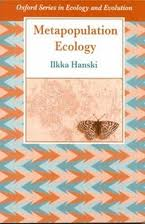
\includegraphics[height=0.7\textheight,keepaspectratio]{figs/metapop-e}
    \hspace{0.3cm}
    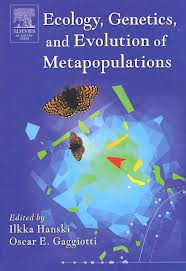
\includegraphics[height=0.7\textheight,keepaspectratio]{figs/metapop-ee}
  \end{center}
\end{frame}



\begin{frame}
  \frametitle{Spatial models}
  \large
  {\bf All else equal\dots}
  \begin{itemize}[<+->]
    \item An unoccupied site should have a higher chance of being
      colonized if it is close to an occupied site than if it is isolated
    \item Similarly, isolated sites should have a higher extinction
      probability than connected sites (rescue effect)
    \item Connectivity is determined by
      \begin{itemize}
        \large
        \item Dispersal ability
        \item Spatial configuration of sites
        \item Landscape resistance to movement
      \end{itemize}
    \item Modern models account for all of this
  \end{itemize}
\end{frame}


% \begin{comment}

% \begin{frame}
%   \frametitle{Colonization functions}
% %  \begin{block}{}%{We need a\dots}
%     \large
%     \begin{itemize}[<+->]
%     \item A function that returns the probability that site
%       $i$ is colonized by a disperser from site $j$, given the
%       distance between them ($d_{i,j}$)
%     \item These functions have at least 2 parameters.
%       \begin{itemize}
%         \large
%         \item $\gamma_0$ is the probability of being colonized by an
%           adjacent neighbor
%         \item $\sigma$ controls how quickly colonization probability
%           declines with the distance between two sites
%         \item Note: The other site must be occupied
%       \end{itemize}
%     \end{itemize}
% %  \end{block}
% %  \pause
% %  \vspace{0.5cm}
% %  \large
% %  {\bf Example}
% %  \begin{itemize}[<+->]
% %    \item Negative exponential: $\gamma_{i,j}=\gamma_0\exp(-d_{i,j}\sigma)$
% %    \item Gaussian: $\gamma_{i,j}=\gamma_0\exp(-d_{i,j}^2/(2\sigma^2))$
% %  \end{itemize}
% \end{frame}


% \begin{frame}[fragile]
%   \frametitle{Gaussian colonization function}% with $\gamma_0=0.6$, $\sigma=1$}
%   The probability that site $i$ is colonized by site $j$ is given by:
%   \[
%     \gamma_{i,j}=\gamma_0\exp(-d_{i,j}^2/(2\sigma^2))
%   \]
% <<nexp0,include=FALSE,echo=FALSE,fig.width=8,fig.height=6>>=
% par(mai=c(0.9, 0.9, 0.1, 0.1))
% sigma <- 1
% gamma0 <- 0.6
% plot(function(x, sig=sigma, gam0=gamma0) gam0*exp(-x^2/(2*sig^2)), 0, 5,
%      xlab="Distance between sites i and j", ylab="Probability of being colonized", #main="1D",
%      cex.lab=1.5, col="cyan3", lwd=3, ylim=0:1)
% @
% <<nexp1,include=FALSE,echo=FALSE,fig.width=12,fig.height=6>>=
% par(mfrow=c(1,2), mai=c(0.9, 0.9, 0.1, 0.1))
% sigma <- 1
% gamma0 <- 0.6
% plot(function(x, sig=sigma, gam0=gamma0) gam0*exp(-x^2/(2*sig^2)), 0, 5,
%      xlab="Distance", ylab="Probability of being colonized", #main="1D",
%      cex.lab=1.5, col="cyan3", lwd=3, ylim=0:1)
% @
% <<nexp2,include=FALSE,echo=FALSE,fig.width=12,fig.height=6>>=
% par(mfrow=c(1,2), mai=c(0.9, 0.9, 0.1, 0.1))
% sigma <- 1
% plot(function(x, sig=sigma, gam0=gamma0) gam0*exp(-x^2/(2*sig)), 0, 5,
%      xlab="Distance", ylab="Probability of being colonized", #main="1D",
%      cex.lab=1.5, col="cyan3", lwd=3, ylim=c(0,1))
% n <- 50
% P <- matrix(0, n, n)
% x <- seq(-5, 5, length=n)
% for(i in 1:n) {
%     for(j in 1:n) {
%         d <- sqrt(x[i]^2 + x[j]^2)
%         P[i,j] <- gamma0*exp(-d^2/(2*sigma^2))
%     }
% }
% persp(x, x, P, zlim=c(0, 1),
%       xlab="Easting", ylab="Northing",
%       zlab="Probability of being colonized",
% #      main="2D",
%       theta=30, phi=20,
%       cex.lab=1.5,
%       ticktype="detailed", col="cyan3")
% @
% %\only<1 | handout:0>{\includegraphics[width=\textwidth]{metapop-nexp1}}
% %\only<2>{\includegraphics[width=\textwidth]{metapop-nexp2}}
% \vfill
% \centering
% \uncover<2>{\includegraphics[width=0.8\textwidth]{metapop-nexp0}} \par
% \end{frame}






%% \begin{frame}[fragile]
%%   \frametitle{Gaussian model with $\gamma_0=0.6$, $\sigma=2$}
%% <<nexp3,fig=TRUE,include=FALSE,echo=FALSE,width=12,height=6>>=
%% par(mfrow=c(1,2), mai=c(0.9, 0.9, 0.1, 0.1))
%% sigma <- 2
%% gamma0 <- 0.6
%% plot(function(x, sig=sigma, gam0=gamma0) gam0*exp(-x^2/(2*sig^2)), 0, 5,
%%      xlab="Distance", ylab="Probability of being colonized", #main="1D",
%%      cex.lab=1.5, col="cyan3", lwd=3, ylim=0:1)
%% n <- 50
%% P <- matrix(0, n, n)
%% x <- seq(-5, 5, length=n)
%% for(i in 1:n) {
%%     for(j in 1:n) {
%%         d <- sqrt(x[i]^2 + x[j]^2)
%%         P[i,j] <- gamma0*exp(-d^2/(2*sigma^2))
%%     }
%% }
%% persp(x, x, P, zlim=c(0, 1),
%%       xlab="Easting", ylab="Northing",
%%       zlab="Probability of being colonized",
%% #      main="2D",
%%       theta=30, phi=20,
%%       cex.lab=1.5,
%%       ticktype="detailed", col="cyan3")
%% @
%% \includegraphics[width=\textwidth]{metapop-nexp3}
%% \end{frame}




% \begin{frame}
%   \frametitle{From pairwise to overall colonization probability}
%   \large
%   {\bf We need to remember some basic probability rules}
%   \begin{itemize}[<+->]
%     \item What is the probability of throwing \textit{at least} one
%       head out of 3 coin tosses?
%     \item In colonization setting, we ask ``what is the probability of
%       being colonized by at least one neighbor?''
%     \item \alert{The answer}: One minus the product of the
%       probabilities of not being colonized by each neighbor.
%   \end{itemize}
% %  \begin{block}{The answer}
% %    One minus the product of the probabilities of not be colonized by
% %    each neighbor
% %  \end{block}
%   \pause
%   \[
%     \gamma_{i,t} = 1 - \left\{\prod_{j=1}^N 1 - \gamma_{i,j}\right\}
%   \]
% \end{frame}


% \begin{frame}
%   \frametitle{Update the non-spatial model}
%   \Large
%   \[
%     \psi_{i,t+1} = O_{i,t}(1-\varepsilon) + (1-O_{i,t})\gamma_{i,t}
%   \]
%   \[
%     O_{i,t+1} \sim \mbox{Bernoulli}(\psi_{i,t+1})
%   \]
% \end{frame}



% \begin{frame}
%   \frametitle{Rescue effect}
%   \Large
%   We could use a similar model for $\varepsilon$ to dampen extinction
%   probability for ``connected'' sites
% \end{frame}


% \begin{frame}
%   \frametitle{Landscape resistance to movement}
%   \Large
%   \begin{itemize}[<+->]
%     \item So far, we have assumed distance is Euclidean
%     \item Animals often prefer to move according to ``least-cost''
%       distance rather than Euclidean distance
%     \item Least-cost distance can be modeled as a function of
%       landscape features
%   \end{itemize}
% \end{frame}



% \begin{frame}
%   \frametitle{Other possible extensions}
%   \Large
%   \begin{itemize}[<+->]
%     \item All parameters can be modeled as functions of habitat
%       variables or environmental stochasticity
%     \item We could switch back from occurrence to abundance
%   \end{itemize}
% \end{frame}


% \end{comment}


\section{Case study}



\begin{frame}
  \frametitle{Case study}
  \begin{columns}
    \begin{column}{0.5\textwidth}
      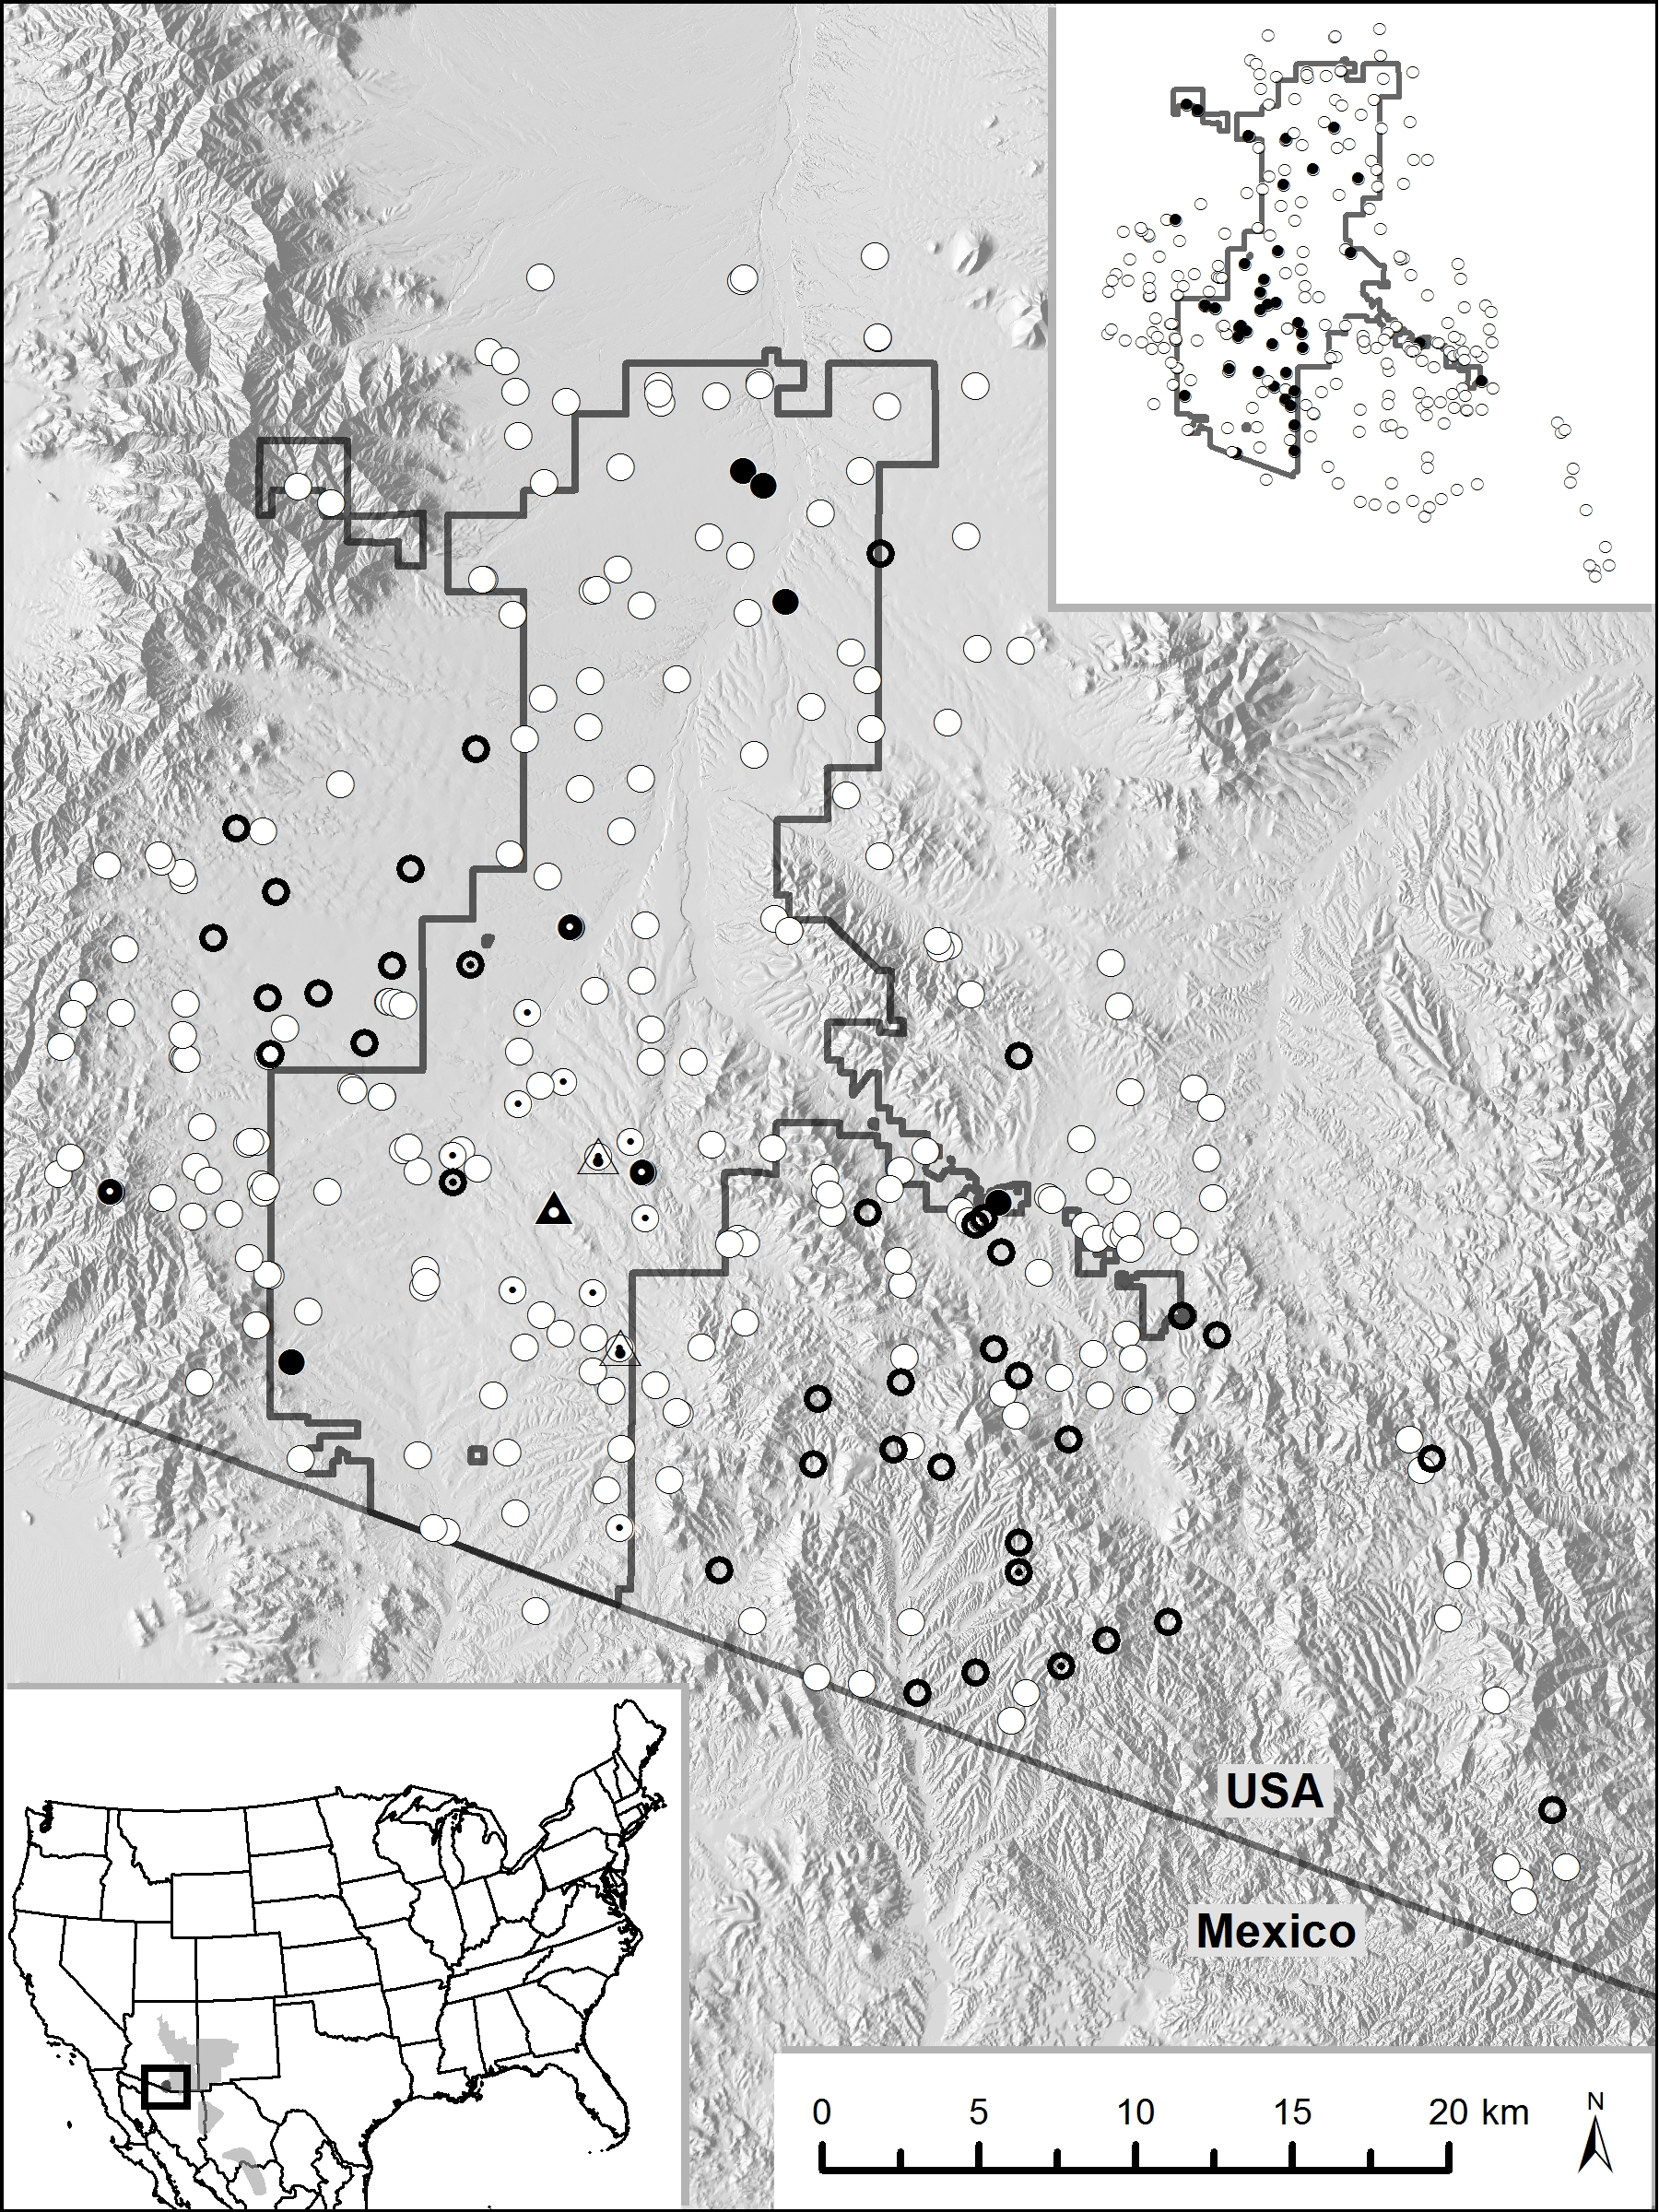
\includegraphics[width=\textwidth]{figs/Altar}
    \end{column}
    \begin{column}{0.5\textwidth}
      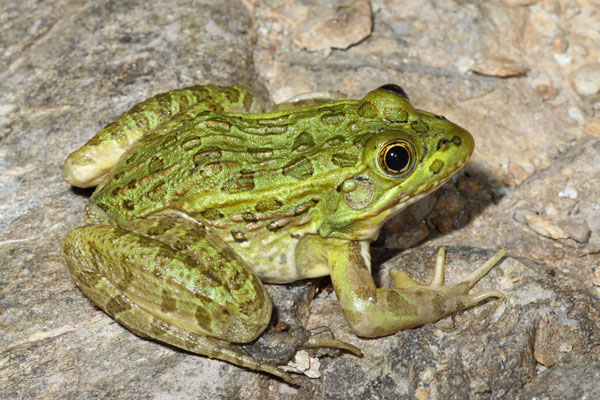
\includegraphics[width=\textwidth]{figs/lich} \\
      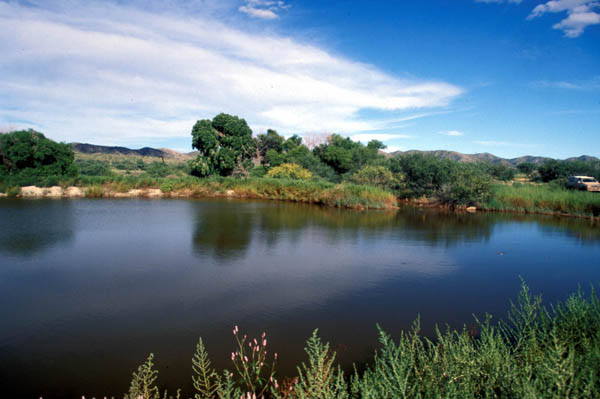
\includegraphics[width=\textwidth]{figs/Carpenter}
    \end{column}
  \end{columns}
\end{frame}




\begin{frame}
  \frametitle{Results}
  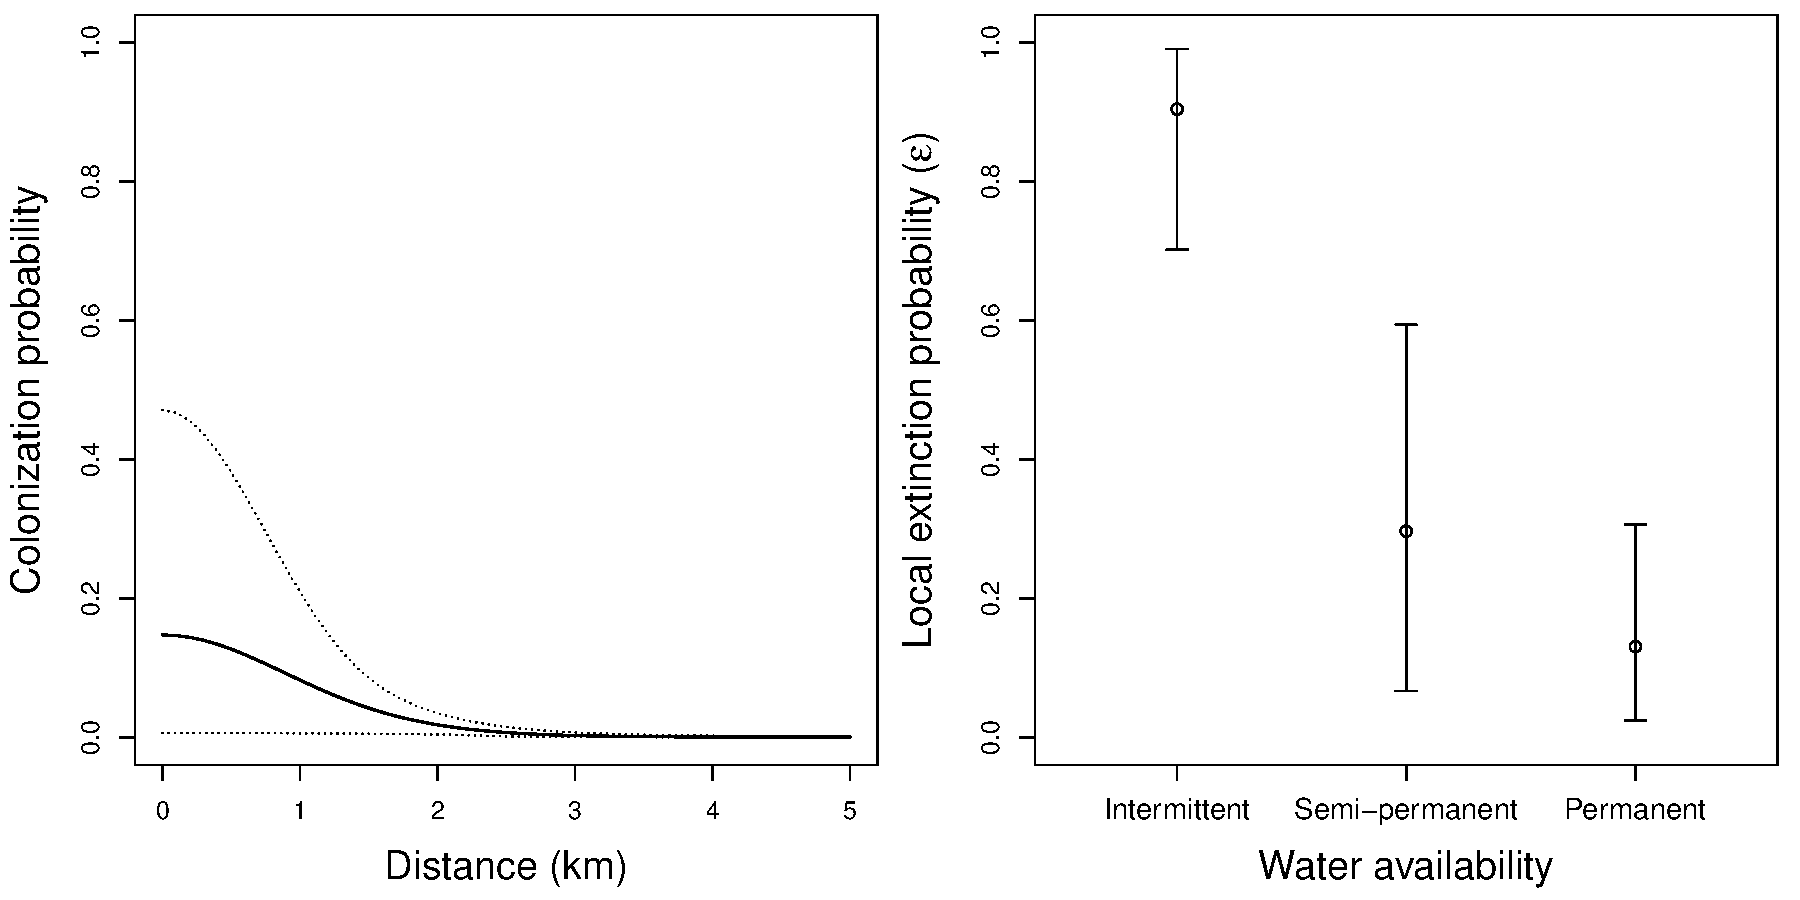
\includegraphics[width=0.95\textwidth]{figs/col-ext} \\
\end{frame}



\begin{frame}
  \frametitle{Results}
  \begin{columns}
    \begin{column}{\textwidth}
      \centering
      \animategraphics[loop,controls,width=0.65\textwidth]{1}{figs/colMap}{2004}{2012} \\
    \end{column}
  \end{columns}
\end{frame}



\begin{frame}
  \frametitle{Results}
  \begin{center}
    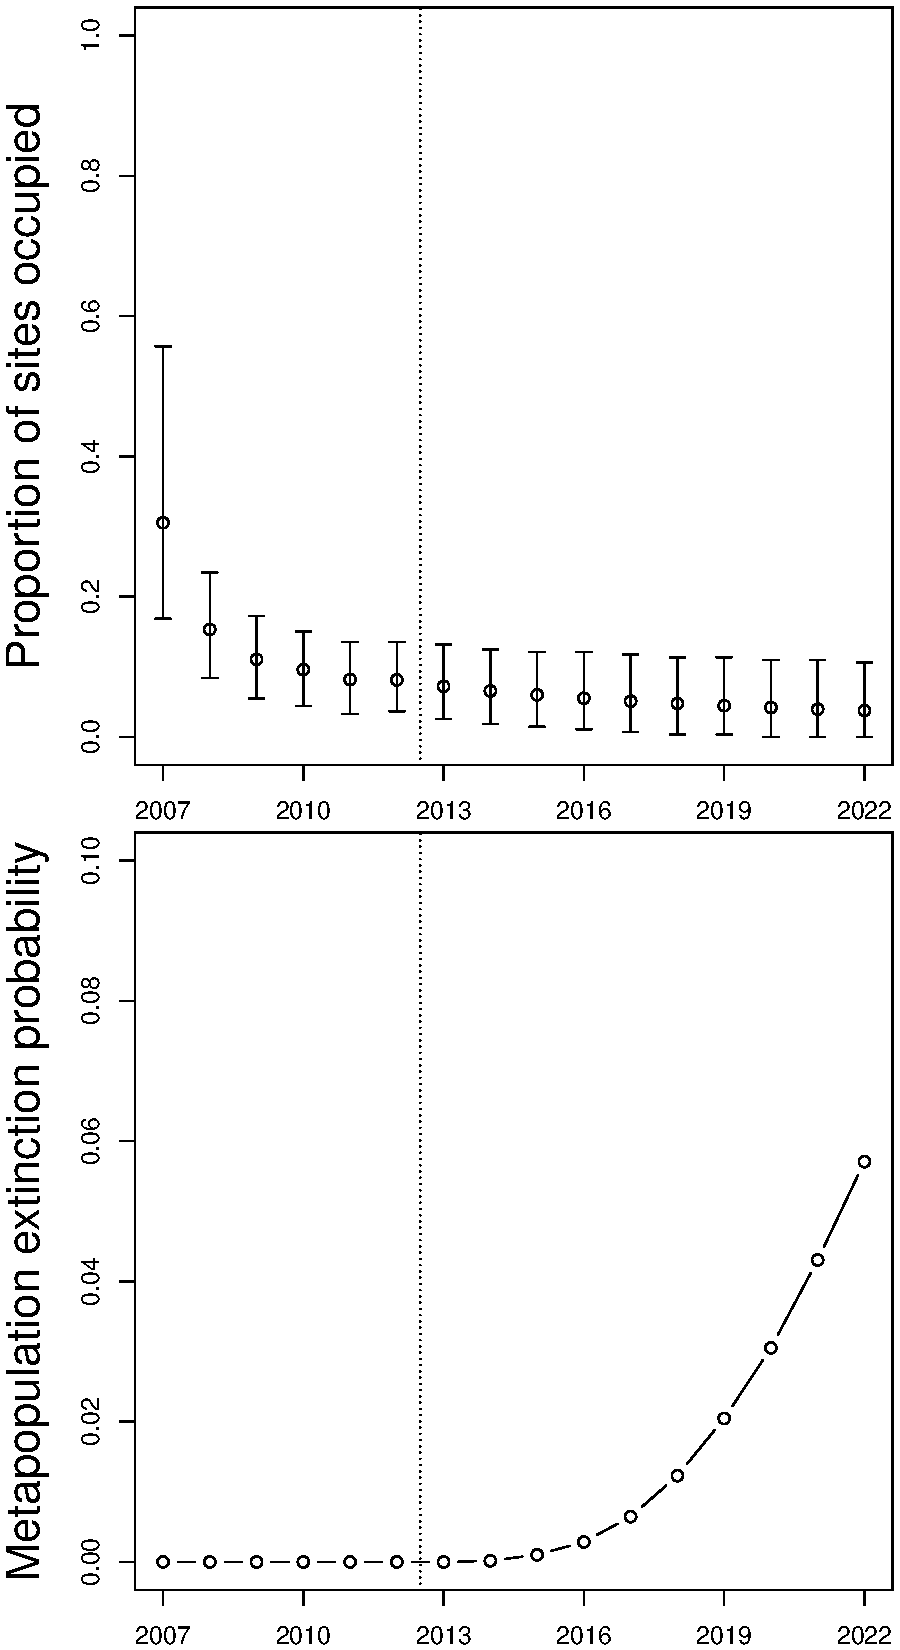
\includegraphics[width=0.38\textwidth]{figs/proj-ext2} \\
  \end{center}
\end{frame}




\begin{frame}
  \frametitle{Summary}
  \large
  Metapopulation models are widely used to describe the
      dynamics of fragmented populations \\
  \vfill
  Model can be formulated in terms of patch-level abundance
      and/or occupancy \\
  \vfill
  Modern models are stochastic and spatially explicit
\end{frame}



\end{document}



